\section{The benchmark}
\label{sec:benchmark}

\subsection{Vocabulary}
\label{sec:notation}

Five terms recur, and it is worth fixing them before they are used.

\begin{center}
\footnotesize
\begin{tabular}{@{}lp{0.66\textwidth}@{}}
\toprule
\textbf{Term} & \textbf{Meaning in this paper} \\
\midrule
\emph{harness} (or \emph{substrate})
  & The agent framework: the software that wraps a language model and turns it
    into something that can read files, run commands and iterate. We compare
    four. It is not the model. \\
\emph{access level}
  & How much pre-written help the agent is given, from \Lzero{} (a scripted
    policy, no model at all) to \Lthree{} (write everything yourself).
    Section~\ref{sec:ladder}. \\
\emph{the contract}
  & The fixed set of machine-checkable conditions every condition's output must
    satisfy: the files exist, the report parses, the predictor runs and returns
    the right shape on the right grid. Section~\ref{sec:contract}. \\
\emph{the frozen set}
  & Sixty solved equilibria, fixed once and never regenerated, on which every
    predictor in this paper is scored. No agent ever sees them. \\
\emph{honesty gap}
  & An agent's own reported error minus its independently measured error.
    Negative means it claimed to be better than it was.
    Section~\ref{sec:honesty}. \\
\bottomrule
\end{tabular}
\end{center}

\subsection{What the agent is asked to do}
\label{sec:task}

Each agent receives a frozen, versioned problem statement --- the same text for
every replicate, hashed into every run record, and reproduced verbatim in
Appendix~\ref{app:tasktext}. It specifies five things.

\textbf{The forward problem.} Fixed-boundary equilibria of D-shaped plasmas in
the five parameters of Section~\ref{sec:physics}, over the stated ranges, at the
solver's default profile shapes.

\textbf{A campaign structure with a hard budget.} At most 150 solves for an
initial space-filling design, then up to three adaptive rounds of exactly 100
new solves each. Failed solves count against the budget. Crucially, each round's
points must be chosen from the current model or the data collected so far: a
single large one-shot design is explicitly ruled out, because the object of
study is the choice of where to sample.

\textbf{A stopping criterion.} Keep a validation set separate from the test set,
and stop early once validation error falls to $0.30\times$ the mean-predictor
baseline or better.

\textbf{An honest evaluation requirement.} Hold out at least 20 solves at random
parameters with a recorded seed, and never use them for training, model
selection or acquisition.

\textbf{A self-assessment requirement.} Report whether the adaptive sampling
actually helped, ``or an honest statement that it did not''.

Four process gates are mandatory and identical for every condition: a
\emph{meshing milestone} (reproduce the solver's own worked example before
generalising), a \emph{pilot gate} (at least 20 solves at 50\% success before
the rounds begin), a \emph{storage-validation gate} (a solve counts as
successful only once its stored file has been read back and confirmed to contain
finite numbers), and a \emph{deliverable self-test} (run every documented
command in a fresh process before declaring done). The last two were added after
an earlier campaign in which an agent stored all-\texttt{NaN} data, counted it as
success, and shipped a predictor it had never executed.

\subsection{The deliverable contract}
\label{sec:contract}

Every condition emits the same three files --- \code{report.json},
\code{predict.py}, \code{README.md} --- and they are checked mechanically
(Table~\ref{tab:gates}). \code{contract.passed} is the flat \textsc{and} of
every gate: no weighting, no partial credit.

\begin{table}[t]
\caption{The deliverable contract. The scoring subprocess is stripped of
provider credentials, so \code{predict.py} must work offline, and it runs in its
own process group so a timeout reaps the solver's children too. The final gate
applies only at \Lthree{}, so \Lthree{} runs face nine checks and \Ltwo{}
eight.}
\label{tab:gates}
\footnotesize
\begin{tabular}{@{}ll@{}}
\toprule
\textbf{Gate} & \textbf{What it checks} \\
\midrule
\code{artifact:report.json} & present and non-empty \\
\code{artifact:predict.py}  & present and non-empty \\
\code{artifact:README.md}   & present and non-empty \\
\code{report\_parses}       & \code{report.json} is valid JSON \\
\code{report\_keys}         & the required keys are \emph{present} \\
\code{predict\_runs}        & \code{python predict.py -{}-input p.json -{}-output o.npz} exits 0 \\
\code{predict\_shape}       & the returned \code{psi} is $(N, 96, 64)$ \\
\code{predict\_grid}        & the returned \code{R}, \code{Z} match the frozen axes to $10^{-9}$ \\
\code{no\_autotokamak\_import} & \Lthree{} only: no workspace file imports the platform library \\
\bottomrule
\end{tabular}
\end{table}

One design choice in that table does a great deal of work later.
\code{report\_keys} \textbf{checks that the agent's self-reported metrics are
present, and never that they are correct}. The agent's own numbers are recorded
verbatim and never cross-checked by the contract. That is what makes the
honesty measurement of Section~\ref{sec:honesty} possible at all: we can compare
what the agent said about itself against what we measured, precisely because
nothing in the pipeline ever forced the two to agree.

Predictions are scored on the frozen set of 60 parameter vectors described in
Section~\ref{sec:physics}, using Equation~\eqref{eq:rell2}. One detail matters:
\textbf{a \texttt{NaN} prediction at a point where the truth is defined is
scored as a full-magnitude miss}, never skipped. Skipping would let an
all-\texttt{NaN} prediction score as perfect.

\subsection{The scaffolding ladder}
\label{sec:ladder}

The benchmark's second axis is how much help the agent gets. All four rungs emit
the identical contract and are scored on the identical frozen set, which is what
makes them comparable at all.

\begin{center}
\footnotesize
\begin{tabular}{@{}llp{0.52\textwidth}@{}}
\toprule
\textbf{Level} & \textbf{Name} & \textbf{What the agent does} \\
\midrule
\Lzero{}  & scripted         & Nothing. A seeded heuristic policy drives a pre-written pipeline; no language model is involved at any point. \\
\Lone{}   & structured       & A model makes only typed decisions --- which model family, how many components, what to do next --- inside fixed pipeline code. \\
\Ltwo{}   & library-assisted & The agent writes the glue code and \emph{may} import the platform library, which already implements the sweep, the acquisition strategies and the model zoo. \\
\Lthree{} & from-scratch     & The agent writes everything. Importing the platform library is forbidden, and the prohibition is audited by static analysis of every file it wrote. \\
\bottomrule
\end{tabular}
\end{center}

\Lzero{} is the reference point that makes the rest interpretable. It is
deterministic, it costs nothing, and it is scored by the same scorer on the same
cases. Without a zero-model condition inside the same contract there is no way
to say how much of a given score is the task being easy and how much is the
agent being good.

\subsection{Is the task hard for the right reasons?}
\label{sec:characterisation}

Before asking whether agents can do this, it is worth establishing that the
task rewards the thing we claim it rewards. Three facts, established by a
direct sweep of 9993 converged solves independent of any agent, are shown in
Figure~\ref{fig:taskchar}; the underlying tables are in
Appendix~\ref{app:characterisation}.

First, error falls with training-set size and saturates --- and \emph{the best
model family changes along the way}, from polynomial ridge up to $N=200$ to
kernel ridge from $N=400$ on. Model selection is therefore a real decision that
depends on the data the agent chose to collect, not a fixed answer that can be
looked up. The agents' 450-solve budget sits in the part of that curve where it
still matters.

Second, at a matched budget, \emph{where} you sample beats \emph{how much}.
Space-filling designs beat uniform random by 21\% at $N=100$, narrowing to 6\%
by $N=1600$; deliberately clustered sampling is catastrophic at every budget.
Coverage is the first-order concern and its value decays as the budget grows.

Third, and this is what makes the sampling decision consequential rather than
cosmetic: \emph{outside its training region the surrogate collapses}. Train on
half the parameter space and test on the other half and the error ratio is
$0.94$ --- no better than predicting the mean field --- against $0.38$--$0.40$
within distribution. An agent that samples badly does not lose a few percent.
It produces a model that fails completely off-distribution and, because it
evaluates itself on its own test set drawn from its own sampling distribution,
it may never find out.

\begin{figure}[t]
\centering
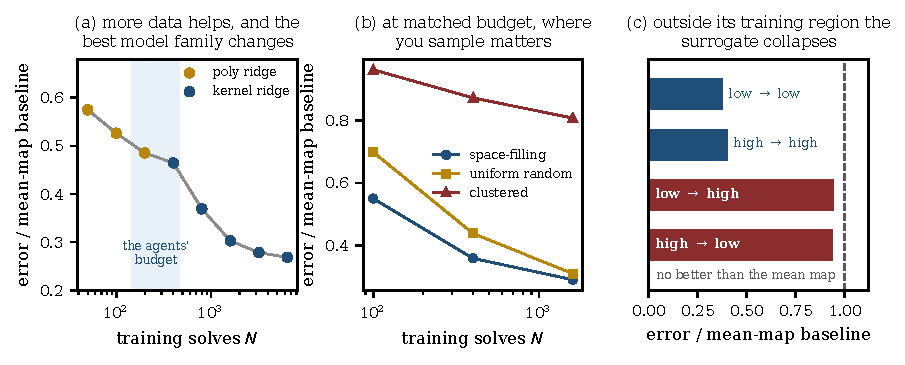
\includegraphics[width=\textwidth]{figures/fig_task_character}
\caption{The task is hard for the right reasons. \textbf{(a)} Error against
training-set size, with the best model family at each size marked; the shaded
band is the agents' campaign budget. \textbf{(b)} At matched budget, sampling
strategy dominates. \textbf{(c)} Trained on one half of the parameter space and
tested on the other, the surrogate is no better than the mean map. All values
are relative $L_2$ divided by the mean-map baseline, from a pool of 9993
converged solves.}
\label{fig:taskchar}
\end{figure}

\subsection{A worked example}
\label{sec:worked}

To make the loop concrete, here is one run end to end:
\Lthree{}-\hn{cursor} replicate~2, chosen because it is unremarkable --- it sits
in the middle of its cell and nothing went wrong.

It received the task text of Section~\ref{sec:task} and a workspace containing
nothing but a read-only copy of the solver's source tree. It began, as
instructed, by locating the solver's own fixed-boundary example and reproducing
it as a standalone script (\code{meshing\_milestone.py} in its workspace),
confirming it could produce a finite flux field before writing anything of its
own. It then built a mesh-and-solve wrapper, ran a 20-solve random pilot to
check the failure rate against the mandated 50\% threshold, and extended to 150
attempted solves with a Latin hypercube over the five parameters. It set aside
a further 30 solves for validation and 25 for its own held-out test, and
recorded a separate seed for each of the four.

For the model it chose something no prompt suggested: a PyTorch multilayer
perceptron mapping the five parameters directly to the $96\times64$ field,
trained under a loss masked to the points inside the plasma. It left dropout
active at inference so that repeated forward passes give a spread, and used
that spread as its acquisition signal --- sampling where the dropout ensemble
disagreed most. One adaptive round of 100 solves was enough: validation error
crossed the task's $0.30\times$-baseline threshold and it stopped early, having
used 305 of its 450 permitted solves.

It wrote the three required files, re-ran its own \code{predict.py} in a fresh
process as instructed, and declared itself done after 8.9 minutes and about
\$1.64 of model spend. Our independent scoring found \relltwo{} $0.0622$ ---
87.4\% accuracy against the mean-map baseline, the fourth-best run in the
campaign. All nine gates passed, all four physical-validity diagnostics passed,
and its \texttt{NaN} mask agreed with ground truth on 99.98\% of grid points.
Its own report claimed $0.0611$ against our $0.0622$: a gap of $-0.001$, which
is to say it flattered itself by a tenth of a percent. It also volunteered,
unprompted, that its adaptive round had helped --- $0.085$ before, $0.061$
after.

That is what the benchmark looks like when everything works. Much of the rest of
this paper is about the runs where it did not, and about how little the contract
noticed.
